\documentclass{beamer}
\usepackage{amssymb} % Therefore symbol
\usepackage{hyperref} % URLs
\title[Critical Thinking 5]{Critical Thinking \\Evaluating risk}
%\subtitle[short]{full}
\author{Andy J. Wills}
\institute[Plymouth University]{School of Psychology\\Plymouth University, U.K.}
\titlegraphic{
\includegraphics[width=.2\textwidth]{plym_logo.png}}


\begin{document}

\frame{\titlepage}
% Welcome to the last critical thinking lecture of the term. Today, how to evaluate risk.

\begin{frame}{Smoking and risk}
\begin{itemize}
%http://upload.wikimedia.org/wikipedia/commons/3/3b/Smoking_kills.png
\centerline{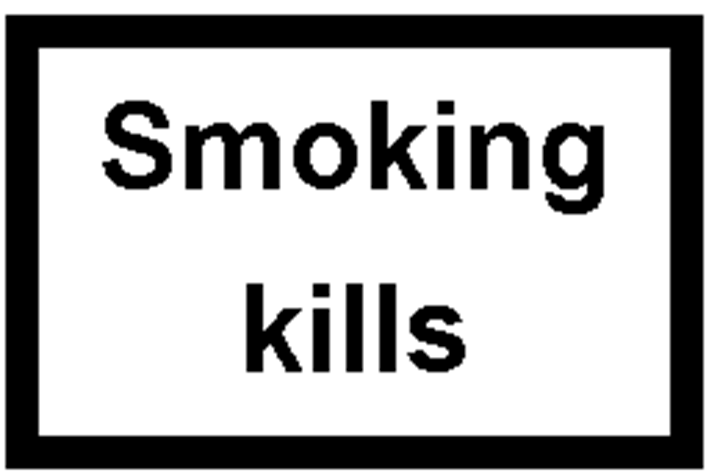
\includegraphics[width=0.5\textwidth]{smokingkills.png}}

\item ``We all gotta die of something''
\item  $P(death|smoker) = 1$
\item  $P(death|nonsmoker) = 1$
\item  How about ``smokers die younger?''

\end{itemize}
\end{frame}

% Let's start with the well-known fag packet warning ``Smoking kills''
% The warning itself - taken literally - must be wrong. It's true that the probability of death,
% given you smoke is 1. The probability of death, given you do not smoke, is also 1. 
% So, your probability of death is unrelated to whether you smoke.
% The daft wording of the warning makes the not uncommon defense:
% ``We all gotta die of something'' entirely reasonable.

\begin{frame}{Smokers die younger (than non-smokers)}
\begin{itemize}
%http://upload.wikimedia.org/wikipedia/commons/thumb/6/64/Cigar_smoking_woman_in_Cuba.jpg/800px-Cigar_smoking_woman_in_Cuba.jpg

\centerline{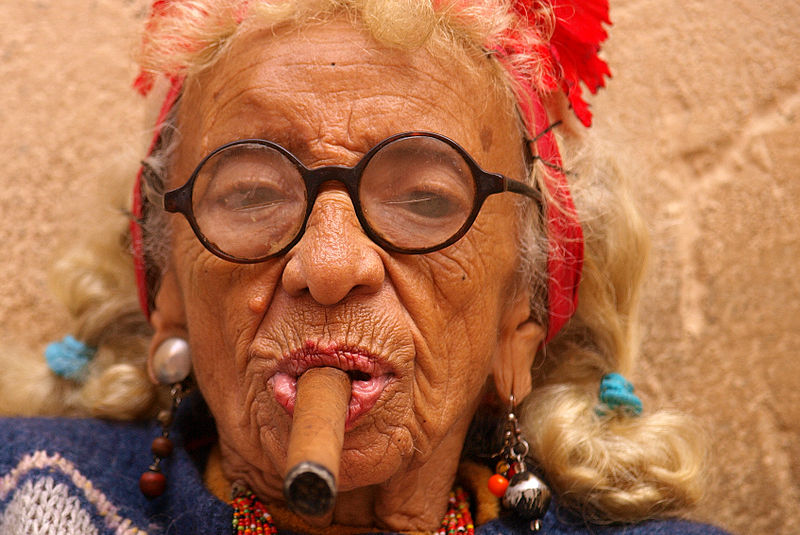
\includegraphics[width=0.5\textwidth]{oldwomansmoking.jpg}}

\item ``I knew a lady who smoked every day, and she lived until she was 93''

\item If the claim is ``ALL smokers die younger than ALL non-smokers''...
\item ...then this counter-example refutes it.
\item Perhaps:
\begin{itemize}
\item ``On average, smokers die younger than non-smokers''
\item ``Smokers have lower life expectancy''
\end{itemize}
\end{itemize}
\end{frame}

% Perhaps a better warning would be ''Smokers die younger [than non-smokers]''

% A not uncommon counter-argument is ``I knew a lady who smoked every day, and she lived until she was 93''

% This counter-argument, although often ridiculed, is also reasonable if one reads the warning as deterministic. In other words, ALL smokers die younger than ALL non-smokers. If that were the argument, the counter-argument would disprove it, because we know lots of people don't make it to 93. 

% The fag packet warning is still ambiguous. What it really means is something like:

% ``On average, smokers die younger than non-smokers'' OR
% ``Smokers have lower life expectancy''

\begin{frame}{Smokers have lower life expectancy}
\begin{itemize}

\item 20\% of smokers die before they are 60 years old 
\item Doll et al.,2004. - Smoking habits of 34000 doctors born 1900-1930.

\item Convinced?
\item Any other information you need?
\end{itemize}
\end{frame}


% OK, how would we go about supporting this clearer claim with data. What if I told you?
% ``20% of smokers die before they are 60''. 
% Are you convinced? What else do you need? 

\begin{frame}{Smokers have lower life expectancy}
\begin{itemize}

\item Think in terms of \emph{hits} and \emph{false alarms}
\item You know $P(DeathBeforeSixty|smoker) = 0.2 $ (hit rate)
\item You also need to know $P(DeathBeforeSixty|nonsmoker)$ (false alarm)
\item $P(DeathBeforeSixty|nonsmoker) = 0.1 $ (Doll et al., 2004)
\end{itemize}
\end{frame}

% What you have is called a hit rate. You also need what's called a ``false alarm'' rate. If 10% of non-smokers die before they are 60, too, then smoking does not affect life expectancy (at least, prior to 60)


\begin{frame}{Odds ratio}
\begin{itemize}

\item $P(DeathBeforeSixty|smoker) = 0.2 $ 
\item $P(DeathBeforeSixty|nonsmoker) = 0.1 $ 
\item Odds ratio, $OR = 0.2 / 0.1 $
\item $OR = 2$
\item Smoking doubles the risk of dying before sixty. 
\end{itemize}
\end{frame}

% ``Yeah, but you could give up smoking and then get hit by a bus''

\begin{frame}{Life is risky}
\begin{itemize}
% http://commons.wikimedia.org/wiki/File:Ljubljana_car_crash_2013.jpg
\centerline{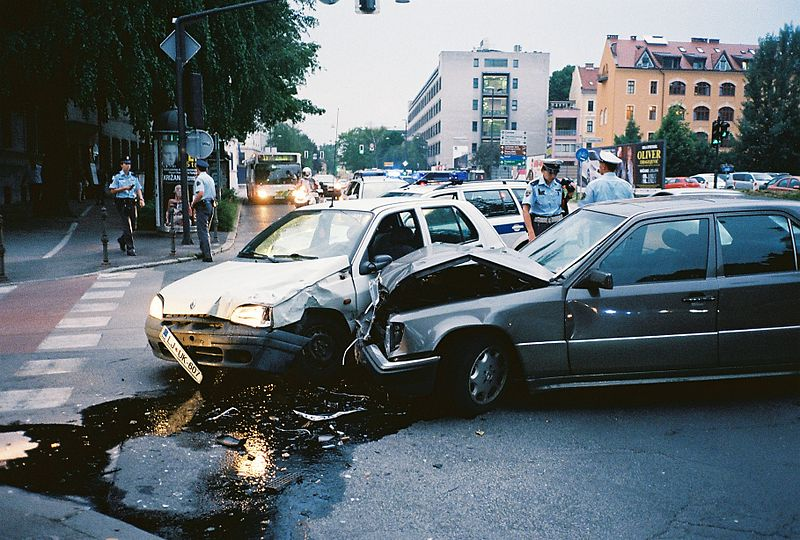
\includegraphics[width=0.5\textwidth]{carcrash.jpg}}
\item ``Yeah, but you could give up smoking and then die in a car accident''
\item ...which possibly means...
\begin{itemize}
\item Many activities have some level of risk.
\item It is impossible to avoid all risk.
\item So everything has to be a risk-benefit analysis otherwise you'd never do anything.
\end{itemize}
\end{itemize}
\end{frame}

% Many activities have some risk. It is impossible to avoid all risk. So everything has to be a risk-benefit analysis otherwise you'd never do anything. 

\begin{frame}{Life is risky? Yes, it is!}
\begin{itemize}
\item Correct. Life is a risk-benefit analysis.
\item Benefit is somewhat subjective - what are the benefits of being a smoker? Or a car driver?
\item ...but odds ratio can help quantify and compare risk.
\end{itemize}
\end{frame}

%http://en.wikipedia.org/wiki/List_of_preventable_causes_of_death
\begin{frame}{Odds ratio}
\begin{itemize}
\item Mokdad et al. (2004) - USA data
\begin{itemize}
\item Tobacco smoking is the cause of death for about 18\% of people.
\item Car accidents are the cause of death for about 0.2\% of people.
\end{itemize}
\item $OR = 18/0.2 = 90$
\item Smoking is 90 times more likely to kill you than driving a car. 
\item Much more than that, actually, because only a minority smoke in the US, but most adults drive regularly.
\end{itemize}
\end{frame}

%http://commons.wikimedia.org/wiki/File:Two_legged_FREAK_(3397831871).jpg
\begin{frame}{I am an individual, not a statistic!}
\centerline{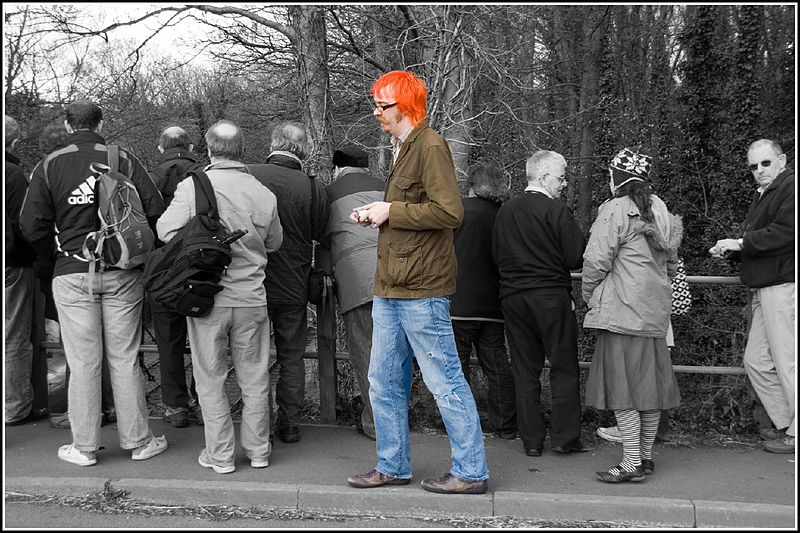
\includegraphics[width=0.5\textwidth]{individual.jpg}}
\begin{itemize}
\item Correct. 
\item These are samples across large numbers of people. They do not \emph{determine} your future cause of death. 
\item But, risk calculations should inform our decisions. Example...
\end{itemize}
\end{frame}

%http://www.telegraph.co.uk/news/9909348/Man-dies-playing-Russian-roulette.html
\begin{frame}{Russian Roulette}
\centerline{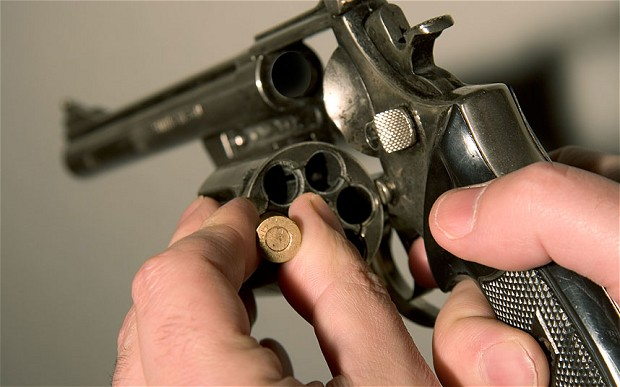
\includegraphics[width=0.5\textwidth]{russianroulette.jpg}}
\begin{itemize}
\item Playing Russian Roulette once, $P(death)= 0.17$
\item After you have played, $P(death) = 1$  or $P(death) = 0$ 
\end{itemize}
\end{frame}

% http://www.flickr.com/photos/terytky/3934371588/sizes/m/in/photostream/
\begin{frame}{Inverse Russian Roulette}
\centerline{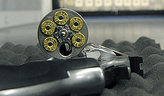
\includegraphics[width=0.5\textwidth]{inverserr.png}}
\begin{itemize}
\item Now imagine \emph{inverse} Russian roulette (five bullets)
\item Playing Inverse Russian Roulette once, $P(death) = .83$
\item Again, after you have played, $P(death) = 1$  or $P(death) = 0$ 
\item If you had to choose between the games, which would you pick ?
\item The odds ratio here is $.83/.17 = 5$ 
\end{itemize}
\end{frame}

% OK, having established that evaluating risk is all about understanding probability, we're going to take a step back and make sure everyone understands the basics of probability.

\begin{frame}{Probability}
\begin{itemize}
\item Probability (by the simplest objective definition) is that property which allows us to calculate the frequency of an event in a very long run of events.

\centerline{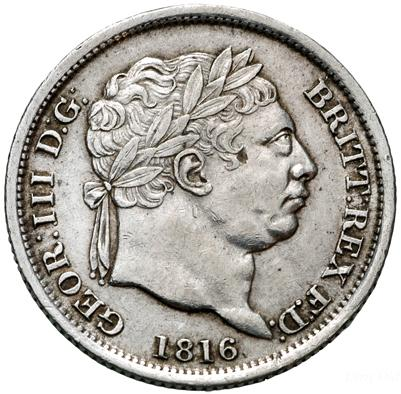
\includegraphics[width=0.2\textwidth]{coin.jpg}}
\item Fair coin 
\begin{itemize}
	\item $P(heads) = 0.5, P(tails) = 0.5$
	\item Flip a fair coin 1000 times, you get close to 500 heads.
	\item The more times you flip the more $heads/flips$ tends towards 0.5.
\end{itemize}
\end{itemize}
\end{frame}

% OK, let's start with the basics. Probability is surprisingly hard to define, but the simplest satisfactory definition is that it allows us to calculate the frequency of an event in a very long run of events.

% So, for example, if I have a fair coin, it can land Heads or Tails, and the probability of each of those events is 0.5. We write this P(heads) = 0.5, P(tails) = 0.5.  If I flip my coin 1,000 times, I would expect to get close to 500 heads. Mathematically: 1000*P(heads) = 1000*0.5 = 500. The more times I flip my coin, the closer the match between the probability and the frequency.

% So, probability of an event is represented P(event) = ..., and the number is always between zero and one.

% As a brief demonstration, estimate the probability of each of these events: 
% Rolling a six on a six-sided dice.
% Having to stand when 60 passengers board a bus with 40 seats.

\begin{frame}{Probability Exercise 1}
\centerline{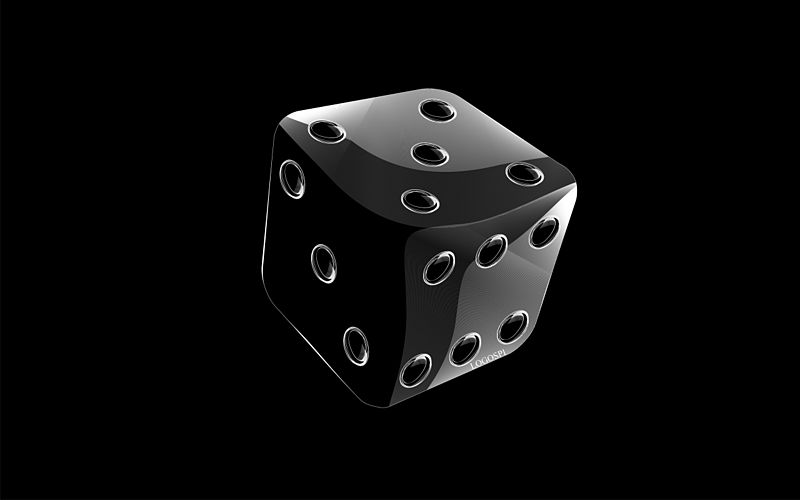
\includegraphics[width=0.4\textwidth]{dice.jpg}}
\begin{itemize}
\item Rolling a six on a six-sided dice.
\item Having to stand when 60 passengers board a bus with 40 seats.
\end{itemize}
\centerline{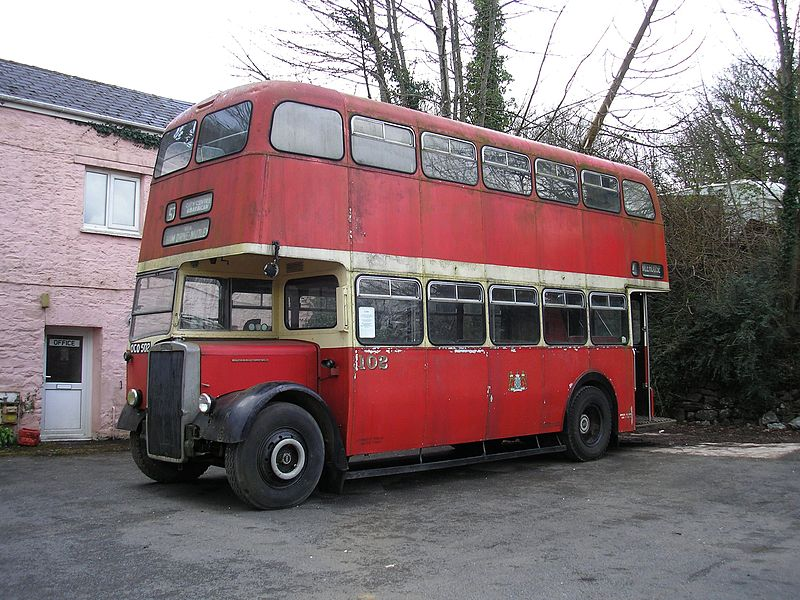
\includegraphics[width=0.4\textwidth]{plymouthbus.jpg}}
\end{frame}

% OK, now how about these:
% Probability of:
% Of dying during 2014, across everyone living in England or Wales (about 0.5%)

% Of getting 4 numbers in the next Lotto game if you buy one ticket (worth around �65). - About 0.1%

% Of committing suicide if you live in England/Wales, are aged 5-34 (about 34% of the population, so about 20 million. About 1000 deaths by suicide in this group - about .005%

\begin{frame}{Probability Exercise 2}
\begin{itemize}
\item Of dying during 2014, across everyone living in England or Wales.
\item Of getting 4 numbers in the next Lotto game if you buy one ticket.
\item Of committing suicide if you live in England/Wales, and are aged 5-34 .
\end{itemize}
\end{frame}

% Statistical independence.

% Basketball players - ask for decisions. (5 min)
% Roulette wheel - ask for decisions. (5 min)
% Winners & losers - ask for estimates. (5 min)


\begin{frame}{Which player would you pass to?}
\centerline{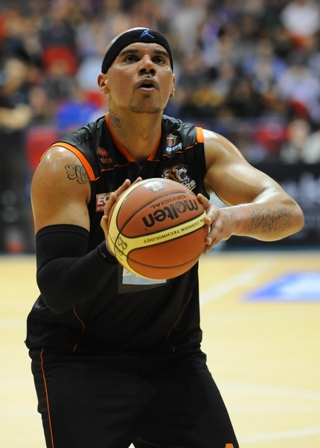
\includegraphics[width=0.4\textwidth]{basketball.jpg}}
\begin{itemize}
\item Player A: Score Score Miss Miss
\item Player B: Miss Miss Score Score
\item A, B, or doesn't matter?
\end{itemize}
\end{frame}

\begin{frame}{Roulette}
\centerline{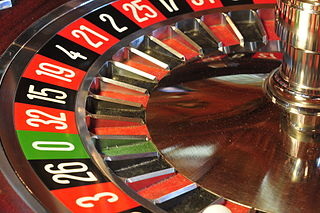
\includegraphics[width=0.8\textwidth]{roulette.jpg}}
\begin{itemize}
\item Red Red Black Red Black Black Black Black 
\item Bet ``red'', bet ``black'', or doesn't matter?
\end{itemize}
\end{frame}

\begin{frame}{Winners and losers}
\begin{itemize}
\item Every day, Adam and Belinda flip a coin.
\item If it comes up heads, Adam keeps the coin.
\item If it comes up tails, Belinda keeps the coin.
\item They do this every day for a year.
\item On any given day, the ``winner'' is the person with the most coins in total. 
\item Estimate the proportion of days on which Adam is a winner.
\item What is more likely?
\begin{itemize}
\item Adam was the winner on 45-55\% of the days.
\item Adam was the winner on 5-15\% of the days. 
\end{itemize}
\end{itemize}
\end{frame}

% Roulette Wheel explanation (5 min)

% Basketball player discussion (10 min)

\begin{frame}{Conditional Probability and Randomness}
\begin{itemize}
\item Probability of some event, given that some other event is known to have occurred.
\item $P(heads_{t}|heads_{t-1}) = 0.5$
\item $P(heads_{t}|tails_{t-1}) = 0.5$
\item Events are \textbf{independent} if the conditional probabilities are equal to the unconditional probabilities (as close to an adequate definition of ``random'' as you're ever likely to get).
\item Coin flips, roulette wheels, etc. are demonstrably independent. 
\end{itemize}
\end{frame}

\begin{frame}{Gamblers' fallacy}
\centerline{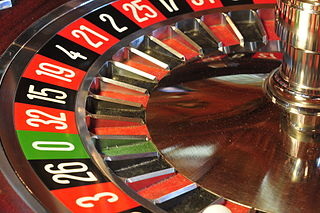
\includegraphics[width=0.4\textwidth]{roulette.jpg}}
\begin{itemize}
\item Red Red Black Red Black Black Black Black 
\item Bet ``red'', bet ``black'', or doesn't matter?
\item Common answer: ``bet red''
\item Rational answers
	\begin{itemize}
		\item If the wheel is known to be unbiased, $P(red) = P(black)$, and it doesn't matter.
		\item From the sample above estimates are that $P(red) < P(black)$, so  bet black.
	\end{itemize}
\end{itemize}
\end{frame}

\begin{frame}{Hot hand fallacy}
\begin{itemize}
\item Player A: Score Score Miss Miss
\item Player B: Miss Miss Score Score
\item A, B, or doesn't matter?
\item Common answer: ``Pass to B'' - Hot Hand fallacy
\item Gilovich, Vallone \& Tversky (1985) - Shots in basketball are independent.
\item Rational answer: Doesn't matter
\item Things to note:
	\begin{itemize}
	\item Basketball experts and players exhibit a hot hand fallacy
	\item Hot Hand and Gamblers' Fallacy are \textbf{opposite} beliefs about independent events. What drives this?
	\end{itemize}
\end{itemize}
\end{frame}

% Winners & losers - demonstration (15 min)
% ... and explanation (5 min)

\begin{frame}{Winners and losers}
\begin{itemize}
\item Every day, Adam and Belinda flip a coin.
\item If it comes up heads, Adam keeps the coin.
\item If it comes up tails, Belinda keeps the coin.
\item They do this every day for a year.
\item On any given day, the ``winner'' is the person with the most coins in total. 
\item Estimate the proportion of days on which Adam is a winner.
\item What is more likely?
\begin{itemize}
\item Adam was the winner on 45-55\% of the days.
\item Adam was the winner on 5-15\% of the days. 
\end{itemize}
\end{itemize}
\end{frame}

\begin{frame}{Winners and losers - Demonstration}
\begin{itemize}
\item Get into pairs. Find a coin.
\item One person flips the coin, the other keeps score (see below).
\item Flip the coin 20 times.
\item Work out proportion of ``days'' on which the ``heads'' is the winner.
\item Write this down. Raise your hand and I'll come to collect your answer.
\end{itemize}
\begin{tabular}{| c | c | c | c | c | }
 \hline
  Throw & Heads or tails? & No. Heads & No. Tails & Winner? \\
 \hline
  1 & H & 1 & 0 & heads \\
  2 & T & 1 & 1 & -- \\
  3 & T & 1 & 2 & tails \\
  ... & & & & \\
  20 & & & & \\
\end{tabular}
\end{frame}

\begin{frame}{Winners and losers}
\begin{itemize}
\item Random events are \textbf{independent}. There is no mechanism that corrects for a run of heads with a run of tails (or vice versa).
\item The \textbf{ratio} of heads to tails approaches 0.5 as we keep flipping the coin. 
\item The \textbf{difference} between the number of heads thrown and the number of tails thrown does not.

\end{itemize}
\end{frame}

% Interlude (10 min)

% Demonstration of regression to mean (10 min).

\begin{frame}{Target game}
\begin{itemize}
\item Target on the floor. 
\item Stand away from the target, with your back to it. 
\item Throw the first coin over your shoulder, try and get as close to the target as possible.
\item Do the same with the second coin.
\item Measure the distance from target for each coin.
\item The two throws are \textbf{independent} events, and there are no appreciable practice effects across two trials.
\item If the first coin is very close to the target, is it more likely that:
\begin{itemize}
	\item The second coin is further away from the target than the first,
	\item The second coin is closer to the target than the first,
	\item Equally likely to be closer or further away.
\end{itemize}
\end{itemize}
\end{frame}

% Regression to the mean

\begin{frame}{Regression to the mean}
\begin{itemize}
\item For \textbf{independent} events, an extreme event at time 1 is likely to be followed by a less extreme event at time 2.
\item This is simply because extreme events are less likely than non-extreme events.
\item Regression to the mean is widely neglected:
\begin{itemize}
\item Evaluation of the efficacy of school inspection programmes, prisoner rehabilitation, treatments for depression...
\item Disappointing post-transfer performance in footballers.
\item Disappointing sequels to great films, books, etc.
\item Why we prefer punishment over reward, even in situations where reward is more effective than punishment.
\end{itemize}
\end{itemize}
\end{frame}

% Summary of independence, and a law of probability

\begin{frame}{Independence - Summary}
\begin{itemize}
\item Events are independent if the probabilities conditional on previous events are equal to the unconditional probabilities:
\item For example: $P(heads_{t}|heads_{t-1}) = P(heads_{t}|tails_{t-1}) = P(heads) = 0.5$
\item Failure to understand independence leads to Gamblers' Fallacy, Hot Hand Fallacy, the ``winners and losers'' fallacy, and a failure to appreciate regression to the mean.
\end{itemize}
\end{frame}




\end{document}
